\chapter{Implementation\label{cha:chapter5}}

This chapter presents the implementation details of the Rollup System, including the chosen technologies, structural decisions, and the encountered development challenges.

\section{Technologies\label{sec:technologies}}

The blockchain components are constructed utilizing the Tezos blockchain\footnote{\url{https://tezos.com/}} and the SmartPy\footnote{\url{https://smartpy.io/}} smart contract language. The Rollup System is deployed on the Tezos Ghostnet test network.

To engineer the Layer 2 components, web servers are developed using nodejs and Typescript running in Docker containers. The implementation of Rollup programs is accomplished through the utilization of the ZoKrates toolbox\footnote{\url{https://github.com/ZoKrates/ZoKrates}}, a comprehensive zk-SNARKs toolkit designed to facilitate the creation of verifiable computation programs.

Those technologies were already decided at the time of the project's inception, as they were the most suitable for the project's objectives. The Tezos blockchain was chosen due to its easy development and deployment, as well as the missing Layer 2 solutions.
\todo[inline]{Write why ZoKrates was chosen}

\section{Enhancing the Scale Tezos Blockchain with Zk-Rollups Project}
This section outlines the implementation of the remaining components in the \textit{Scale Tezos Blockchain using Zk-Rollups} project. Additionally, modifications made to the existing features are explained to accommodate these new enhancements.

\subsection{Storage}

Initially, the storage was designed with the intention of accommodating a limited number of users, employing a standard Map. It encompassed the following elements:
\begin{itemize}
	\item A Map of accounts indexed by a natural number, containing:
		\begin{itemize}
			\item A public key;
			\item A balance.
		\end{itemize}
	\item A list of 8 scalar values representing the Merkle Tree root of the accounts' public keys;
	\item A list of 8 scalar values representing the Merkle Tree root of the accounts' balances.
\end{itemize}

With scalability as a focal point, the storage structure was revamped to handle a growing user base through the adoption of a Big Map. This alteration is pivotal, given that the Big Map is lazily deserialized\footnote{\url{https://tezos.gitlab.io/michelson-reference/\#type-big_map}}, negating the need for gas during contract calls to deserialize the entire accounts Map. The storage now comprises:
\begin{itemize}
	\item A Big Map of accounts indexed by a natural number, encompassing:
		\begin{itemize}
			\item A public key;
			\item A balance;
			\item A nonce.
		\end{itemize}
	\item A list of 8 scalar values representing the Merkle Tree root of the accounts' public keys;
	\item A list of 8 scalar values representing the Merkle Tree root of the accounts' balances concatenated with their respective nonces.
\end{itemize}

Details on the nonce mechanism and the Merkle Tree roots are elucidated in Section \ref{subsec:repeatedtransactionsattack}.

\subsection{Repeated Transactions Attack}
\label{subsec:repeatedtransactionsattack}

To mitigate the risk of an attacker initiating repeated transactions, the nonce mechanism comes into play: each account holds a nonce, stored on Layer 1. When a transaction is submitted, it must include a nonce incremented by one, thereby facilitating the validation of transaction execution history.

Within the ZoKrates environment, proving the usage of updated balances and nonces necessitates computation of a merkle tree for the provided balance and nonce lists. This implies calculating two full binary trees, thereby increasing complexity. A workaround involves concatenating and hashing balances and nonces for individual users, forming a single merkle tree of these concatenated values. This approach incurs only the complexity of the concatenation function, involving a number of hashes equivalent to the number of accounts, ultimately substantiating the updated balances and nonces.

Changes were introduced to the rollup execution to incorporate the computation of new nonces alongside new balances. It's essential that ZoKrates receives transactions ordered by nonce for each user. While transactions from diverse users can be received, those from a single user must be ordered by nonce. The algorithm for verifying transaction nonces and calculating new nonces is as follows:
\begin{itemize}
	\item Generate a new array \textit{X} by copying the old nonce array;
	\item Iterate through the transactions:
	\item \begin{itemize}
		\item Check in \textit{X} if the transaction nonce for the sender equals the user's nonce plus one;
		\item If true, increment the user's nonce in array \textit{X} and proceed;
		\item If false, terminate execution.
    \end{itemize}
\end{itemize}

This approach accommodates multiple transactions from the same user, thwarting duplicate transaction execution.

The rollup execution complexity experiences minimal augmentation, as the nonce check coincides with balance calculation in the same loop, facilitating direct array access and preserving an O(n) complexity.

\subsection{ZoKrates Native Execution}
The execution of ZoKrates programs demands substantial resources, as evidenced in Section \ref{sec:benchmarks}. As a consequence, executing ZoKrates programs is allocated to a distinct server. This server operates as an independent entity, called upon by the primary Web Server. This strategy serves the dual purpose of optimizing resource allocation and facilitating scalability. Specifically, the architecture enables the isolation of resource-intensive tasks to a separate server, allowing efficient utilization and the ability to scale individual components as needed.

The primary server dispatches requests, inclusive of essential inputs sourced from the Manager smart contract, to the ZoKrates servers. These dedicated servers execute the ZoKrates programs, subsequently furnishing the results to the primary server. Notably, the utilization of a containerized environment for the ZoKrates server introduces challenges. The approach of running ZoKrates programs directly on the machine is chosen to mitigate the introduction of overhead stemming from OS-level virtualization, particularly relevant in scenarios involving pre-existing virtualized environments, such as cloud computing contexts. Figure \ref{fig:5_drawings-L2_technologies_ZoKrates_metal} illustrates the technologies of the new Layer 2 components.

\begin{figure}[ht]
	\centering
	\includegraphics[width=0.7\columnwidth]{5_drawings-L2_technologies_ZoKrates_metal.png}
	\caption[Scaling Solutions]{Technologies of the new Layer 2 components.}  
	\label{fig:5_drawings-L2_technologies_ZoKrates_metal}
  \end{figure} 


\section{New Features Implementation}
This section details the implementation of the new features of the project, including the problems encountered and the solutions devised.

\subsection{Registration and Deregistration}

This segment elucidates the registration and deregistration procedures for users. The primary objective is to add and remove users from storage, creating empty user entries during deregistration. This approach maintains user positioning within storage, allowing utilization of existing indexes.

Tezos supports optional types, enabling a value to be set as None, indicating its absence. This feature proves valuable during user removal from storage. The new storage Big Map, representing registered users, now comprises:
\begin{itemize}
	\item \textbf{index}: A natural number representing the user's index within storage;
	\item \textbf{mutez balance}: The user's balance;
	\item \textbf{nonce}: The user's nonce;
	\item \textit{optional} \textbf{public key}: The user's public key.
\end{itemize}

Given the resource-intensive nature of merkle tree generation, registration and deregistration processes are executed within dedicated ZoKrates programs and not in the smart contracts.

\subsubsection{Registration\label{subsec:registration}}

To register a new user, the two Merkle Trees must be recomputed, integrating the new user's public key, balance, and nonce. A ZoKrates program performs this computation, returning the new root hashes of both Merkle Trees. These hashes are then used by the manager smart contract to update the storage, incorporating new roots and the new user. The ZoKrates program requires the precise position for inserting the new user's data. This position is determined externally by a manager, which can communicate with an RPC to ascertain the first vacant slot within the storage's Big Map. The registration process verifies if the designated position holds an account with an empty key, balance, and nonce set to zero. Subsequently, the user's nonce is set to one, balance to zero, and public key to the user's public key.

\subsubsection{Deregistration}

Deregistration closely mirrors the registration process outlined in Section \ref{subsec:registration}. The ZoKrates deregistration program takes the user's index to be deregistered, along with other standard inputs. This program sets the user's public key to None, balance to zero, and nonce to zero. The updated root hashes of both Merkle Trees are returned by the deregistration program. The manager contract then employs these new roots to update storage, removing the user entry at the specified index.

\subsection{Deposit\label{subsec:deposit}}
The deposit process into the Layer 2 system is intricate due to the requirement of recalculating the merkle tree involving balances and nonces. As a result, the deposit procedure is divided into two distinct phases: the initial phase entails transferring funds from the user's account to the manager smart contract via a dedicated entrypoint call in the contract; the subsequent phase involves executing a ZoKrates program to recompute the merkle tree of balances and nonces, ultimately producing the new root of the tree. Figure \ref{fig:5_drawings-sequence_deposit.png} illustrates the deposit process.

\subsubsection{Phase 1: Transferring Funds to Manager Contract}
The deposit process is instigated by the user, who invokes the \textit{deposit} entrypoint within the manager contract and specifies the index of the account within the user Big Map. Subsequently, the manager contract facilitates the transfer of the designated sum from the user's account to its own account. Additionally, an internal record of pending deposits is maintained.

This internal deposit record adopts the structure of a \textit{Map (nat mutez)}, where the key corresponds to the user's index in the user Big Map, and the value signifies the sum of funds intended for deposition. This configuration accommodates the acceptance of multiple deposits from a single user, effectively tracking the specified deposit amounts.

In the aftermath of the first phase, the user remains unable to expend the transferred sum until the conclusion of the second phase.

\subsubsection{Phase 2: Merkle Tree Recalculation}
The second phase is initiated by a Web Server that detects a considerable accumulation of deposits in the deposit queue. Subsequently, the Web Server accesses the deposit list and initiates the ZoKrates program responsible for recalculating the merkle tree inclusive of the new deposits. Following this computation, the Web Server calls the \textit{receive\_deposit\_proof} entrypoint within the manager contract, providing the freshly computed merkle tree root as a parameter. Consequently, the manager contract updates the root of the merkle tree associated with balances and nonces, adjusts user balances to incorporate the deposited funds, and ultimately eradicates the deposits from the internal pending deposit list.

\begin{figure}[ht]
	\centering
	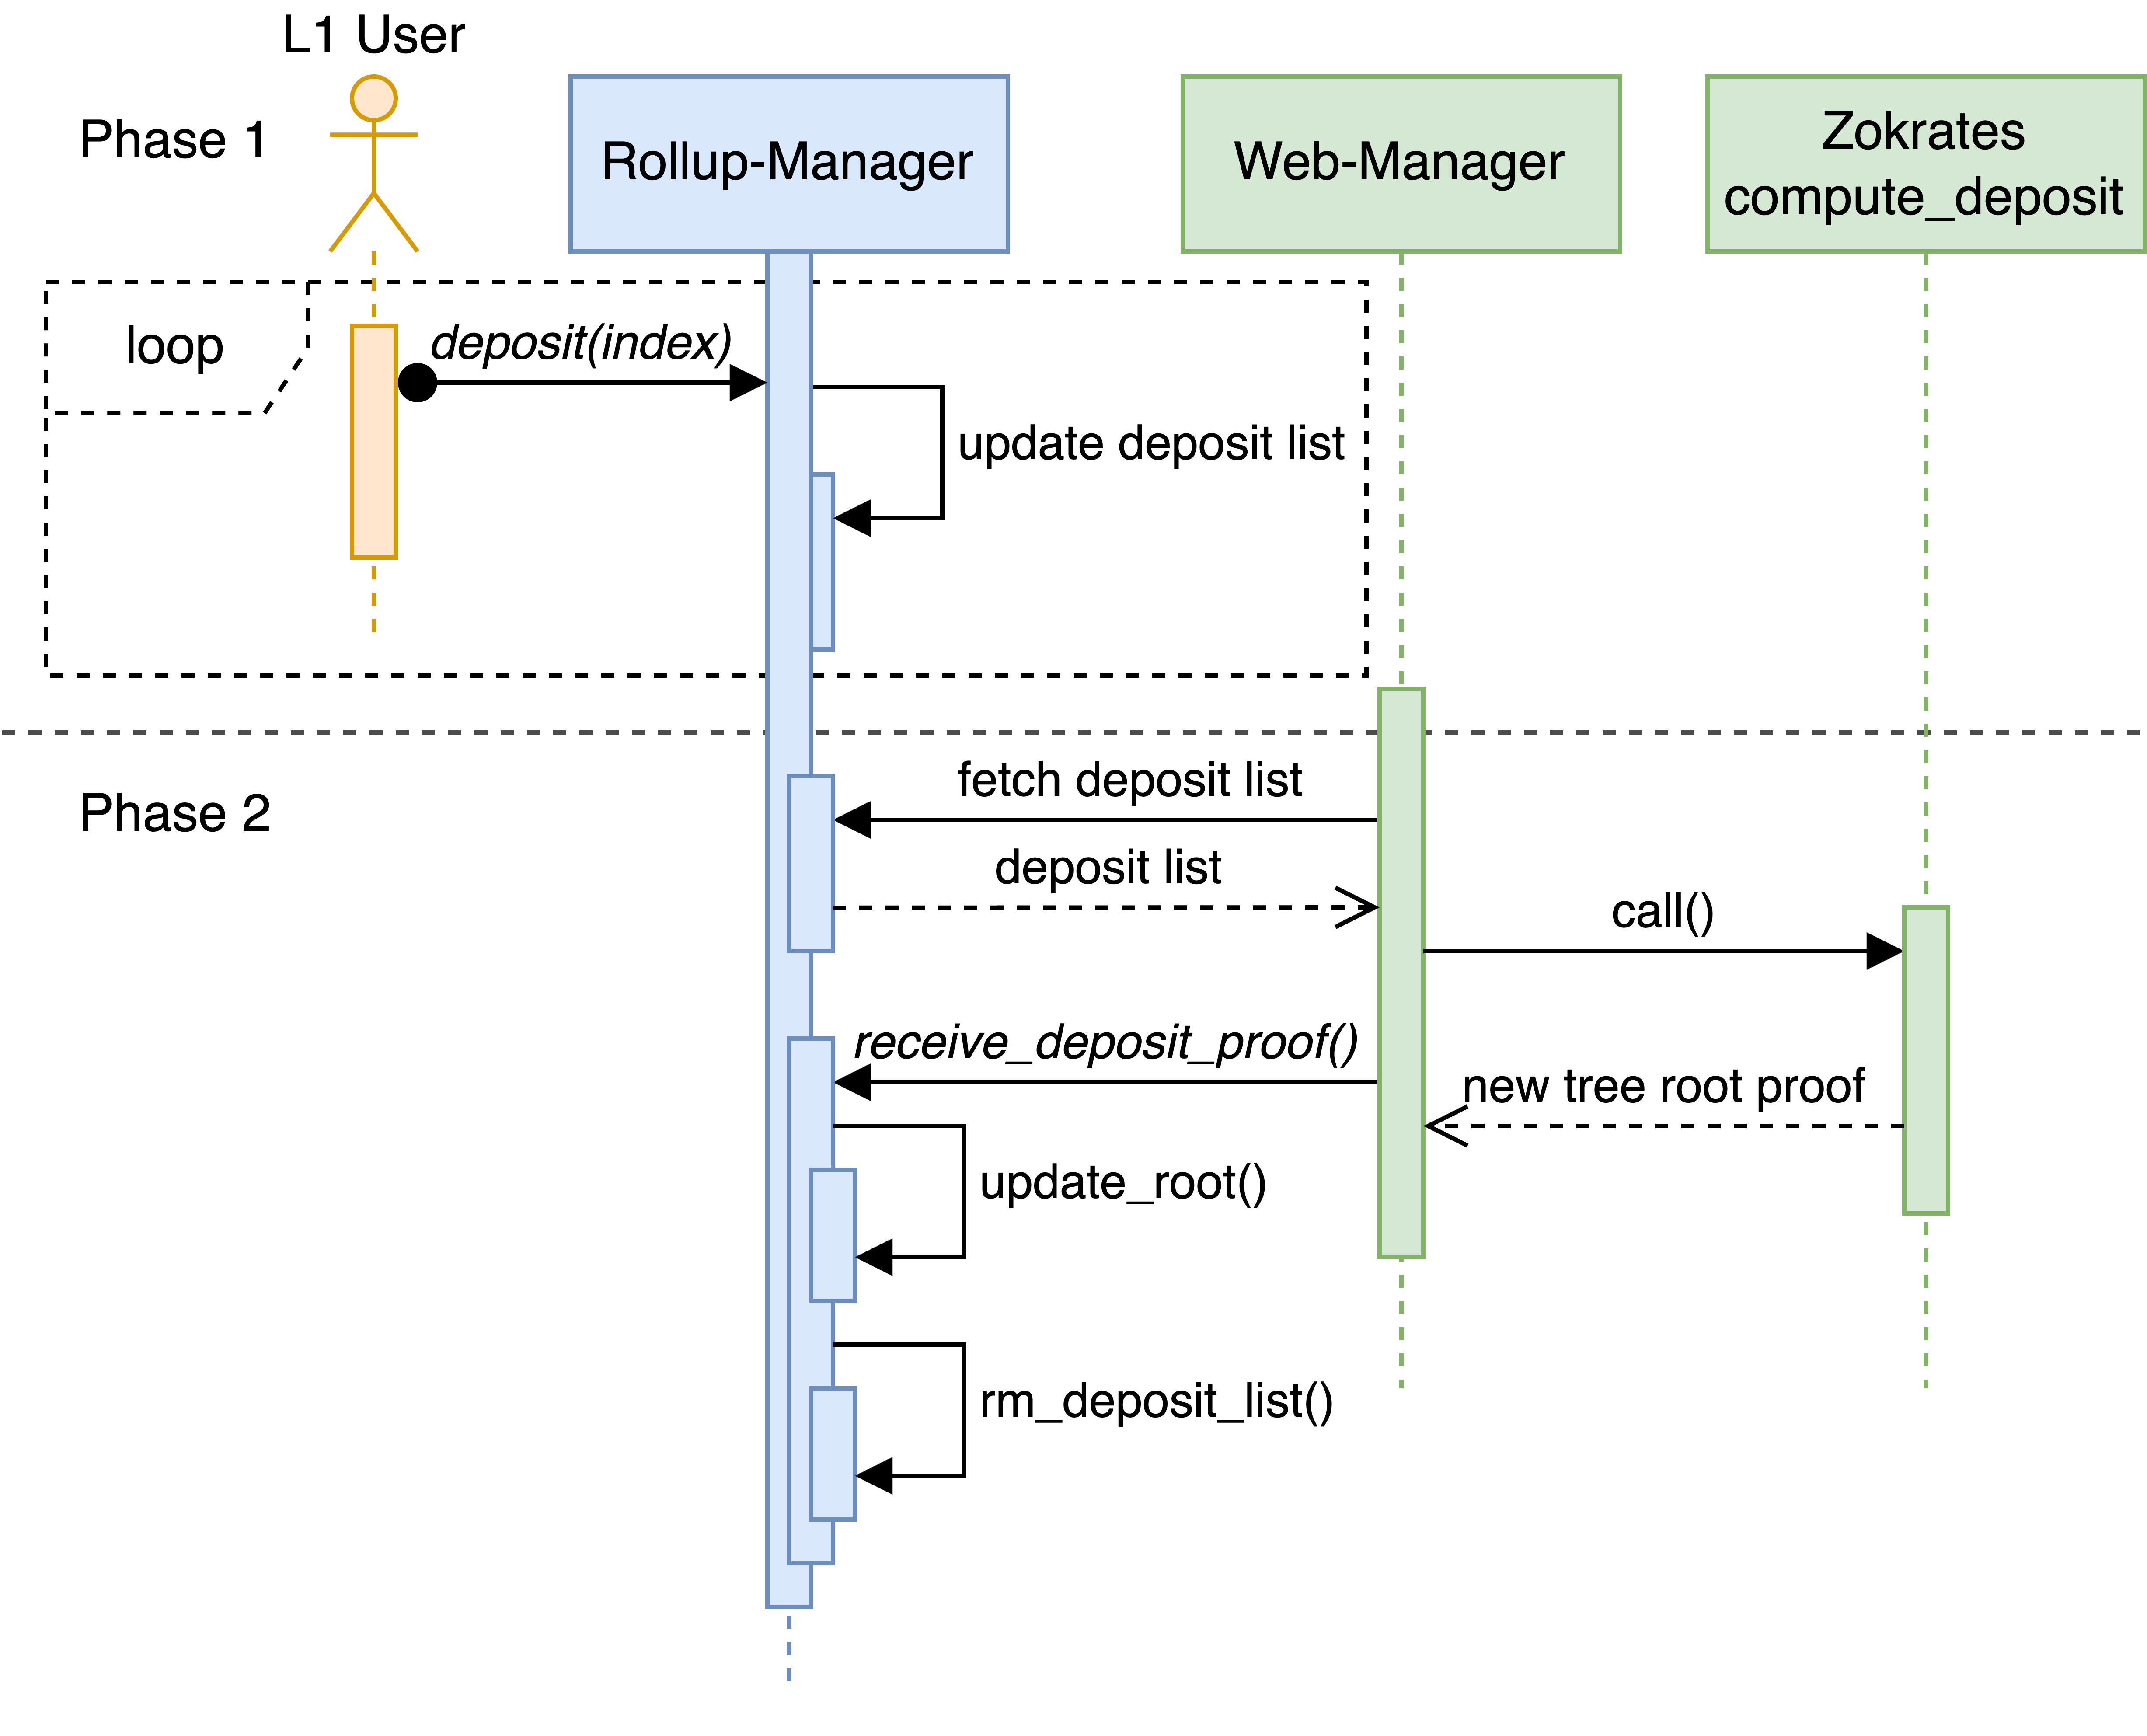
\includegraphics[width=0.7\columnwidth]{5_drawings-sequence_deposit.png}
	\caption[Scaling Solutions]{Sequence Diagram of Deposit Process}  
	\label{fig:5_drawings-sequence_deposit.png}
  \end{figure} 

  \subsection{Withdraw}
  This section delineates the Withdrawal process, enabling the movement of funds from the Layer 2 system to the Layer 1 system. The withdrawal process diverges from the deposit process expounded in Section \ref{subsec:deposit}. Notably, withdrawals operate within a single phase, a strategic choice that expedites the withdrawal procedure, affording users the prompt retrieval of their funds without the necessity of reaching a threshold of users in the withdrawal queue.
  
  The withdrawal initiation commences as users dispatch withdrawal requests to the Web Server. Subsequently, the Web Server retrieves the user's balance and nonce from the manager contract and generates withdrawal inputs for the dedicated ZoKrates program. This ZoKrates program orchestrates the computation of the new root hash for the merkle tree containing balances and nonces. This computation involves the subtraction of the user-specified amount. The computed new root hash is then relayed back to the Web Server. In turn, the Web Server invokes the \textit{receive\_withdrawal\_proof} entrypoint within the manager smart contract. This invocation encompasses the provision of the new root hash as a parameter.
  
  Within the manager contract, the merkle tree root hash undergoes an update, alongside adjustments to the user's balance and nonce. Subsequently, the requested sum is transferred to the user's account, finalizing the withdrawal process.
  


\section{Optimization}
During a preliminary testing phase of the Layer 2 system immediately emerged a problem when increasing the number of user from 4 to 8. The problem was the compute resources needed to compile and run the ZoKrates programs: with only 8 users the compilation of the programs required more than 100GB of RAM. Due to the structure of the merkle trees generation, only powers of 2 can be taken as number of users. The 

\begin{figure}[htb]
  \centering
  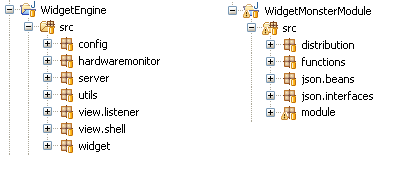
\includegraphics[width=10cm]{screenshot_2_projects}
  \caption{Project Structure}
  \label{fig:projects}
\end{figure}

\noindent
The following listing briefly describes the single packages of both projects in alphabetical order to give an overview of the implementation:
\\
\\
\textbf{config} 
\\
Lorem Ipsum...
\\
\\
\textbf{server} 
\\
Lorem Ipsum...
\\
\\
\textbf{utils} 
\\
Lorem Ipsum...

\section{Important Implementation Aspects\label{sec:implaspects}}

Do not explain every class in detail. Give a short introduction about the modules or the eclipse projects. If you want to explain relevant code snippets use the 'lstlisting' tag of LaTeX. Put only short snippets into your thesis. Long listing should be part of the annex.

\lstset{caption=JSON String Code Snippet,label=jsonstring,showstringspaces=false}
\begin{lstlisting}
{
	id: 1,
	method: "myInstance.getGroup",
	params: ["Teammates", 2, true]
}

{
	id: 2,
	result: [
		  "groupDesc":"These are my teammates",
		  {
			"javaClass":"src.package.MemberClass",
			"memberName": "Bob",      
		  }
		]
}\end{lstlisting}

You can also compare different approaches. Example: Since the implementation based on X failed I choosed to implement the same aspect based on Y. The new approach resulted in a much faster ...

\section{Graphical User Interface\label{sec:gui}}

Lorem Ipsum...

\section{Documentation\label{sec:docu}}

Lorem Ipsum...


